\documentclass{report}
\usepackage{comment}
\usepackage{graphicx} % Required for inserting images
\graphicspath{ {./images/} }
\usepackage{geometry}
\usepackage[T1]{fontenc}
\usepackage{fbb}
\usepackage{amsthm}
\usepackage[libertine]{newtxmath} 
\usepackage[italic]{mathastext}
\MTsetmathskips{f}{5mu}{1mu} 
\usepackage[utf8]{inputenc}
\usepackage{textcomp}
\usepackage{graphicx}
\usepackage{listings}
\usepackage{caption}
\usepackage{fullpage}
\usepackage{caption}
\usepackage{subcaption}
\usepackage{lipsum}
\usepackage[backend=biber]{biblatex}
\addbibresource{refs.bib}
\usepackage{setspace}
\usepackage{chngcntr}
\counterwithout{section}{chapter}
\usepackage{fancyhdr}
\usepackage{titlesec}
\usepackage{listings}
\usepackage{multirow}
\usepackage{scalerel}
\DeclareMathOperator*{\bigplus}{\scalerel*{+}{\sum}}
\usepackage{tikz-cd}
\usetikzlibrary{patterns.meta}
\usepackage{hyperref}
\geometry{hmargin=2.5cm,vmargin=3cm,lmargin=1.75cm,rmargin=1.75cm}
\pagestyle{fancy}
\setlength{\headheight}{12pt}
\fancyhf{}
\fancyhead[L]{\slshape\nouppercase{\leftmark}}
\fancyhead[R]{\slshape\nouppercase{\rightmark}}
\chead{\textsc{Dylan Laird}}
\cfoot{\thepage}
\renewcommand{\headrulewidth}{0.4pt}
\renewcommand{\footrulewidth}{0.4pt}
\renewcommand\contentsname{Summary}
\setlength{\headsep}{1cm}
\addbibresource{refs.bib}
\renewcommand{\chaptername}{Part}
\titleclass{\subsubsubsection}{straight}[\subsection]


\newcounter{subsubsubsection}[subsubsection]
\renewcommand\thesubsubsubsection{\thesubsubsection.\arabic{subsubsubsection}}
\renewcommand\theparagraph{\thesubsubsubsection.\arabic{paragraph}} % optional; useful if paragraphs are to be numbered

\titleformat{\subsubsubsection}
  {\normalfont\normalsize\bfseries}{\thesubsubsubsection}{1em}{}
\titlespacing*{\subsubsubsection}
{0pt}{3.25ex plus 1ex minus .2ex}{1.5ex plus .2ex}

\makeatletter
\renewcommand\paragraph{\@startsection{paragraph}{5}{\z@}%
  {3.25ex \@plus1ex \@minus.2ex}%
  {-1em}%
  {\normalfont\normalsize\bfseries}}
\renewcommand\subparagraph{\@startsection{subparagraph}{6}{\parindent}%
  {3.25ex \@plus1ex \@minus .2ex}%
  {-1em}%
  {\normalfont\normalsize\bfseries}}
\def\toclevel@subsubsubsection{4}
\def\toclevel@paragraph{5}
\def\toclevel@paragraph{6}
\def\l@subsubsubsection{\@dottedtocline{4}{7em}{4em}}
\def\l@paragraph{\@dottedtocline{5}{10em}{5em}}
\def\l@subparagraph{\@dottedtocline{6}{14em}{6em}}
\makeatother

\setcounter{secnumdepth}{4}
\setcounter{tocdepth}{4}
\begin{document}
\newtheorem{mydef}{Definition}[subsection]
\newtheorem{theorem}[mydef]{Theorem}
\newtheorem{prop}[mydef]{Proposition}


\makeatletter
\def\@makechapterhead#1{%
  %%%%\vspace*{50\p@}% %%% removed!
  {\parindent \z@ \raggedright \normalfont
    \ifnum \c@secnumdepth >\m@ne
        \huge\bfseries \@chapapp\space \thechapter
        \par\nobreak
        \vskip 20\p@
    \fi
    \interlinepenalty\@M
    \Huge \bfseries #1\par\nobreak
    \vskip 20\p@
  }}
\def\@makeschapterhead#1{%
  %%%%%\vspace*{50\p@}% %%% removed!
  {\parindent \z@ \raggedright
    \normalfont
    \interlinepenalty\@M
    \Huge \bfseries  #1\par\nobreak
    \vskip 20\p@
  }}
\makeatother

\begin{titlepage}
\newcommand{\HRule}{\rule{\linewidth}{0.5mm}} % Defines a new command for the horizontal lines, change thickness here
\renewcommand{\bibname}{Bibliography and links}
\center % Center everything on the page

%----------------------------------------------------------------------------------------
%	HEADING SECTIONS
%----------------------------------------------------------------------------------------

\textsc{\LARGE École Normale supérieure de Lyon}\\[1cm] % Name of your university/college
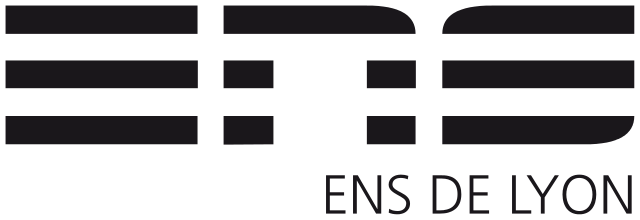
\includegraphics[height=2cm, keepaspectratio]{École_normale_supérieure_de_Lyon_Logo.svg.png}\\[1cm]

\textsc{\LARGE Research Internship report}\\[1.25cm]
\HRule \\[0.4cm]
{ \huge \bfseries The Hypercubic Manifold}\\[0.3cm]
{ \huge \bfseries in}\\[0.5cm] 
{ \huge \bfseries Homotopy Type Theory}\\[0.3cm]
\HRule \\[2cm]
\begin{minipage}{0.4\textwidth}
\begin{flushleft}
\emph{\Large \emph{\textbf{Author :}}}\\[0.2cm]
\textsc{\Large Dylan LAIRD}\\
\textit{Student at ENS Lyon}
\end{flushleft}
\end{minipage}
~
\begin{minipage}{0.4\textwidth}
\begin{flushleft}
\emph{\Large \emph{\textbf{Supervisers :}}}\\[0.2cm]
\textsc{\Large Samuel MIMRAM}\\
\textit{Professor at LIX, École Polytechnique}\\[0.1cm]
\textsc{\Large Émile OLÉON}\\
\textit{PhD student at LIX, École Polytechnique}\\
\end{flushleft}
\end{minipage}\\[0.5cm]

\begin{figure}[h]
    \begin{minipage}[c]{.46\linewidth}
        \centering
        
\includegraphics[height= 5cm]{École_polytechnique_signature.svg.png}
    \end{minipage}
    \begin{minipage}[c]{.46\linewidth}
        \centering
        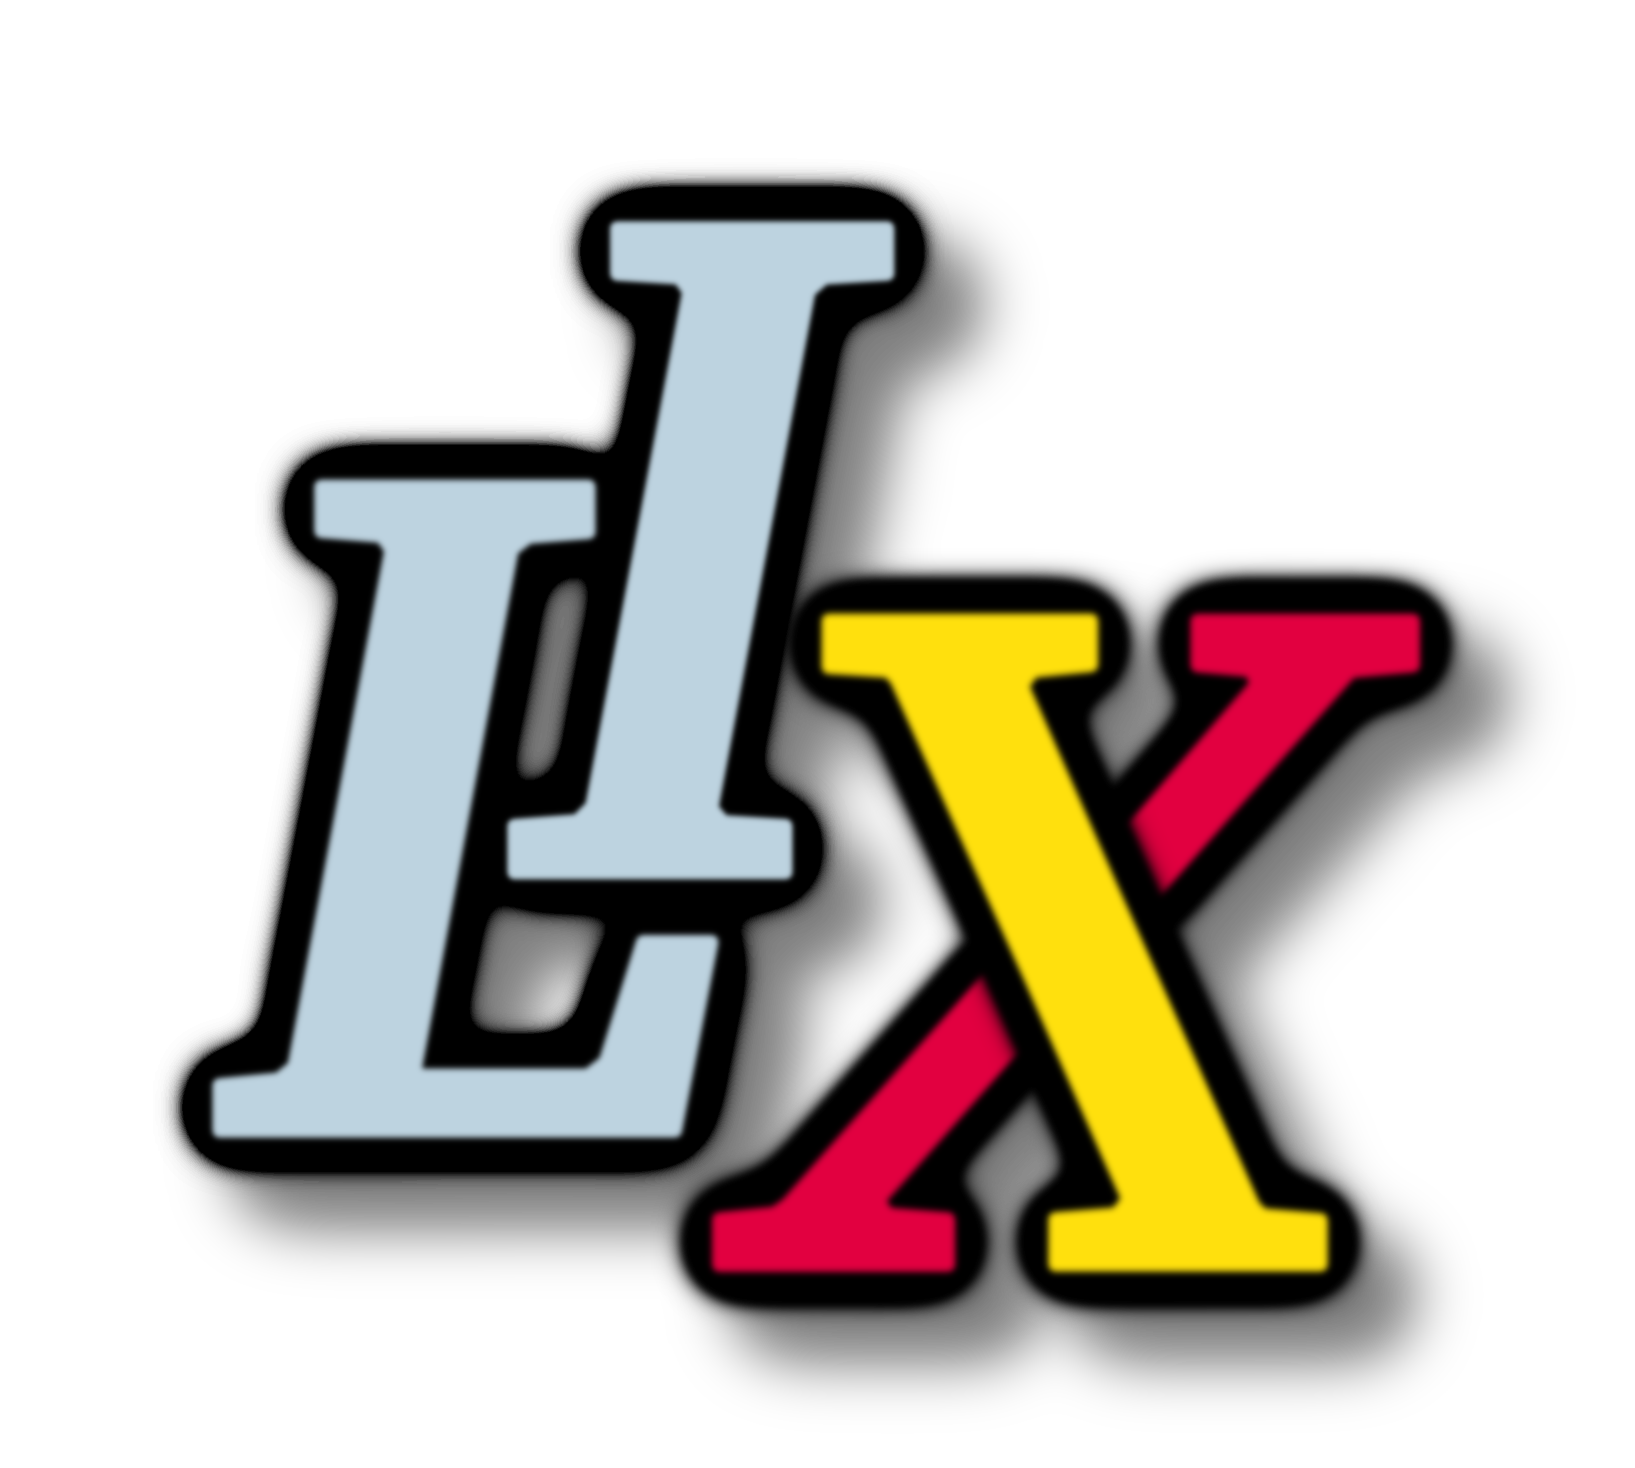
\includegraphics[height=5cm]{logo_lix.png}
    \end{minipage}
\end{figure}
\vfill % Fill the rest of the page with whitespace
\end{titlepage}
\tableofcontents
\section{Introduction}
\textbf{Homotopy Type Theory} (HoTT) is a new field in mathematics and computer science, at the crossroads of \textbf{Type Theory}, \textbf{Homotopy Theory} and the \textbf{Foundations of Mathematics}. It is based on a homotopical interpretation of \textbf{Martin-Löf's type theory}, with the addition of the \textbf{univalence axiom} and \textbf{Higher Inductive Types}. HoTT has seen massive developments as both a candidate for a new foundational system for mathematics, and as a basis for for developing \textbf{synthetic homotopy theory}. Being a constructive type system, it is also implemented in proof assistants such as Agda and Coq. However, since the univalence axiom is not computable,  \textbf{cubical type theory} has emerged in recent years as an alternative to HoTT by giving a constructive interpretation of univalence.\\
The objective of this internship was, first, to define the \textbf{hypercubic manifold} \cite{hypercubic} (historically introduced by Poincaré at the beginning of algebraic topology) in HoTT/cubical type theory using the proof assistant Agda proof, and second, to provide some further results about it that should eventually lead to the definition of a \textbf{cellular delooping of the quaternion group} $\mathcal Q$ (I will explain why this is of interest in Part 2).\\
Homotopy type theory being a very atypical theory, it comes with a lot of new definitions, ideas and concepts. This makes it hard to summarize both the basic theory (roughly speaking, chapters 1,2,3,4,6 and 8 of the \textbf{HoTT Book} \cite{hott}) as well as the new content from the internship itself in 20 pages. For that reason, \textbf{this report (Part 1) will summarize both basic and more advanced topics in HoTT} (although many details and important results will be overlooked due to the space limitations), and the work I did during the internship (Part 2) will not take up the most important portion of space in this report. All the formalized results, and attempts, obtained during the internship can be found on this GitHub repository \cite{repo}.
\chapter{Pre-requesites}
The following part aims to give the reader a sufficent background knowledge  to understand the material from the internship. The presentation is very much inspired by the \textbf{HoTT Book} \cite{hott}. 
\section{Type Theory}
In type theory, all that we manipulate are \textbf{types} $A,B$ and \textbf{terms} of those types for instance $a : A$ and we have \textbf{type forming rules} to form terms of types from already existing types. The most infamous example is the one of the natural integers defined inductively by:
\begin{itemize}
    \item $0 : \mathbb N$
    \item $\mathrm{suc}: \mathbb N \rightarrow \mathbb N$
\end{itemize}
The type of natural integers also comes with its well-known \textbf{induction principle}. In type theory, since all we work with are types, we will also have induction principles that come along with any type we define.\\
It is to be noted that \textbf{equality} plays a central role in Type Theory. We distinguish two kind of equalities, \textbf{definitional equality}, which we will note $\equiv$, it is not an actual part of Type Theory but lives at the same level as judgements "$a : A $". For example, setting $f$ to be the function $x \mapsto x^2 $ (say over the integers), for any integer $a$ we would then have $f a \equiv a^2$, which is to be read as "$f a$ is definitionnally equal to $a^2$".\\
It must not be mistaken with \textbf{(propositional) equality} which we will take a closer look at later on. For now, let's just recall that in Type Theory every object is a type and so, for two elements $a,b :A$ we can build the type $a =_A b$, namely the \textbf{identity type} of $a$ and $b$. To prove that $a$ and $b$ are equal elements (of $A$), one has to produce an element $p : a=_A b$.
\subsection{Function types}
Given two types $A,B$, one can build the \textbf{type} $A \rightarrow B$ of functions from $A$ to $B$. To build an element of that type, one needs to give an expression $\Phi(x)$ such that : $a : A \vdash \Phi(a) : A$, and can define an element $f$ with the following syntax: 
$$f(x) :\equiv \Phi(x) \hspace{5pt}\text{(such definitions yield \textbf{definitional} equalities)}$$
\subsection{Universes, type families and dependent function types}
To introduce types more formally, we need to talk about \textbf{universes}, which, as in set theory, allow us to avoid unsoundness problems (such as the Russel paradox). Details need not concern us here, let's just get straight to the point: we suppose that we have a \textbf{cumulative hierarchy} of universes $\mathcal{U}_i$, and elements of such a universe are themselves some types. Hence, giving ourselves a type $A$ is tantamount to giving ourselves an element from some universe $\mathcal{U}$ (we will not mention the level from now on).\\
 Universes allow us to introduce \textbf{Type families}, that is, a type family over a type $A$ is a function of type $A \to \mathcal{U}$.
 \paragraph{Dependent function types ($\Pi$-types)}
 For now, let's note that we can talk about \textbf{dependent functions}. Given a type $A$ and a type family $C: A \rightarrow \mathcal{U}$, one can build the type of dependent functions over $A$, whose codomain can vary along $C$: 
$$\prod_{x : A} C(x)$$
The formation rule is the same as before, one can build an element $f$ of type $\prod_{x : A} C(x)$ with an expression $\Phi(x)$ such that $a : A \vdash \Phi(a) : C(a)$ and by setting $f(x) :\equiv \Phi(x)$.
\subsection{Product types}
Given types $A,B : \mathcal{U}$ one can build their \textbf{cartesian product type} $A \times B : \mathcal{U}$. The formation rule is as natural as it gets, given $a : A$ and $b : B$ one can form $(a,b) : A \times B$. We shall now encounter our first \textbf{recursion principle}, which in the general case, encompasses how to build \textbf{non-dependent functions} out of a certain type. The recursion principle for product types allows us to define a function over $A\times B$ by specifying its values on pairs $(a,b)$. This principle can be phrased properly in type theory as the following:
$$\mathrm{rec}_{A\times B} : \prod_{C : \mathcal{U}} (A \rightarrow B \rightarrow C) \rightarrow A\times B \rightarrow C$$
with the defining equation:
$$\mathrm{rec}_{A\times B}(C,f,(a,b)) :\equiv f(a)(b)$$ 
From now on, we will only refer informally to the recursion and induction principles without writing them out formally.\\
As an example, we can now define the first projection $\mathrm{pr}_1 : A\times B \rightarrow A$ by $\mathrm{pr}_1(a,b) :\equiv a$ and the second projection by $\mathrm{pr}_2 (a,b) :\equiv b$.\\ 
This brings us to a central philosophical aspect of Type Theory. In classical mathematics, one constructs the product of sets $A$ and $B$ with the sets of all pairs of the form $(a,b)$. In Type Theory however, we have not (yet) seen any mention that the type $A\times B$ is the "type of all pairs $(a,b)$", meaning that there may be some element $x : A \times B$ which is \textit{not} a pair $(a,b)$. In fact, it turns out that we do have a \textbf{uniqueness principle} for product types, which resembles what we could expect, however, as we are working within Type Theory we cannot expect it to be more than a \textbf{propositional uniqueness principle}. Before stating it, we need to take a look at the \textbf{induction principle} for product types, which in the general case encompasses how to build \textbf{dependent functions} out of a certain type. In our case, as for the recursion principle, defining a dependent function $f$ over $A \times B$ only requires defining its value for pairs $(a,b)$.\\
We are now ready to prove the \textbf{propositional uniqueness principle of product types} :
\begin{prop}
  For any $x : A \times B$, one has : $x =_{A \times B} (\mathrm{pr}_1(x),\mathrm{pr}_2(x))$, that is, we have a dependent function:
  $$\mathrm{uniq}_{A\times B} : \prod_{x : A \times B} \big(x =_{A \times B} (\mathrm{pr}_1(x),\mathrm{pr}_2(x))\big)$$
\end{prop}
\begin{proof}
     Here, we want to build the dependent function $\mathrm{uniq}_{A\times B}$. We will hence be using the induction principle for product types, which states that we need to exhibit for any pair $a : A$ and $b:B$ an element$f(a)(b)$ of type $(a,b)=_{A \times B} (\mathrm{pr}_1((a,b)),\mathrm{pr}_2(a,b))$. However,  $(\mathrm{pr}_1((a,b)),\mathrm{pr}_2(a,b))$ is \textbf{definitionally} equal to $(a,b)$ (by the definition that we have given of the projections) and so we are reduced to exhibit $f(a)(b) : (a,b)=_{A \times B} (a,b)$.\\ 
     We shall now use a fact that we have not seen yet about identity types, but that should seem familiar, which is that for any $x$ of some type $X$ the type $x=_{X}x$ is inhabited by an element $\mathrm{refl}_x$. We can therefore set $f(a)(b) :\equiv \mathrm{refl}_{(a,b)}$ to terminate the proof.
\end{proof}
\subsection{Dependent pair types ($\Sigma$-types)}
Given a type $A$ and a type family $B : A \rightarrow \mathcal{U}$, one can construct the \textbf{dependent pair type}: 
$$\sum_{x : A} B(x)$$
To form an element of such a type, one needs elements $a : A$ and $b : B(a)$, resulting in an element $(a,b) : \sum_{x : A} B(x)$. It should be noted that theses types are a generalisation of product types and that for the constant type family at $B$, $C :\equiv \lambda (x : A).B$ we have $\sum_{x = A} C(x)\equiv A \times B$.\\
As for product types, one can define dependent and non dependent functions $f$ over the type $\sum_{x : A} B(x)$ by specifiying its values on dependant pairs $(a,b)$ where $b:B(a)$.\\ 
The recursion principle allows us to define (again) the first projection $\mathrm{pr}_1 : \sum_{x : A} B(x) \rightarrow A$ by $\mathrm{pr}_1 (a,b) :\equiv a$.\\
However, defining the second projection is a bit trickier since it should have the type $\prod_{p : \sum_{x : A} B(x)} \mathrm{pr}_1(p)$, making it a dependent function. It thus requires the use of the induction principle, and we can define it by its values on dependant pairs by $\mathrm{pr}_2(a,b) :\equiv b$.
\subsection{Coproduct types}
Given types $A$ and $B$, one can define their coproduct type $A+B$ inductively with two constructors:
\begin{itemize}
  \item inl : $A \rightarrow A+B$
  \item inr : $B \rightarrow A+B$
\end{itemize}
It should be thought of as containing two disjoints copies of $A$ and $B$. The induction principle is here tantamount to \textbf{case analysis}, to define a function over $A+B$ one needs to specify its value on elements $inl(a)$ for $a:A$ and on elements $inr(b)$ for $b:B$. 
\subsection{Propositions as types}
\begin{figure}[h]
\begin{center}
\begin{tabular}{|c|c|}
\hline Types & Logic  \\
\hline$A$ & $A$ is a proposition  \\
\hline$a: A$ & $a$ is a proof of $A$ \\
\hline $\textbf{0},\textbf{1}$ & $\perp, \top$ \\
\hline$A+B$ & $A \vee B$  \\
\hline$A \times B$ & $A \wedge B$  \\
\hline$A \rightarrow B$ & $A \Rightarrow B$ \\
\hline$A \rightarrow \textbf{0}$ & $\lnot A$ \\
\hline
\end{tabular}
\end{center}
\end{figure}
The propositions as types correspondence shows the similarity between type forming rules and rules of propositional logic when seeing "propositions as types" and vice versa. For instance, if one wants to build a term of type $A \times B$, one needs a term $a : A$ and a term $b : B$ to form $(a,b) : A \times B$. Similarly, to prove the proposition $A \land B$, one needs a proof of $A$ and a proof of $B$. \\
In the same way, building a function $f : A \rightarrow B$ (or a proof of $A \implies B)$ requires to be able to build an element of $B$ (a proof of $B$) given an element an $A$ (given a proof of $A$).\\
Under this correspondence, it also makes sense to talk about a predicate over a type $A$ for a type family $P : A \rightarrow \mathcal{U}$. Then, for $a :A$ the type $P(a)$ corresponds to the propositions "$P$ holds for $a$". We then have the following correspondence : 
\begin{center}
  \begin{tabular}{|c|c|}
  \hline Types & Logic  \\
  \hline$\prod_{x : A} P(x)$ & For all $x :A$, $P(x)$ holds  \\
  \hline$\sum_{x : A} P(x)$ & There exists $x : A$ such that $P(x)$ holds\\
  \hline
  \end{tabular}
\end{center} 
One can also think of the type $\sum_{x: a} P(x)$ as the type of all $x : A$ such that $P(x)$ holds.
\paragraph{Semi-groups}
Let's illustrate how our type formers and the proposition as types interpretation allow us to define mathematical structures . We call a \textbf{semigroup} a type $A$ equipped with an associative binary operation $m : A \times A \rightarrow A$. Under the proposition as types interpretation, the proposition that $m$ is associative is given by the following type : 
$$\mathrm{isAssoc}(m) : \prod_{x,y,z : A }m(x,m(y,z))=m(m(x,y),z)$$
Then, a semigroup structure is given by a type $A$, a binary operation $m$ over $A$ and a proof that $m$ is associative, and so we can the define the type of semigroups over a universe $\mathcal{U}$ by : 
$$\mathrm{SemiGroup} :\equiv \sum_{A : \mathcal{U}} \sum_{m : A \times A \rightarrow A} \mathrm{isAssoc}(m)$$
\subsection{Identity types family}
For a type $A: \mathcal{U}$ we have a type family $\mathrm{Id} : A \rightarrow A \rightarrow \mathcal{U}$ (we will write $x=y$ for $\mathrm{Id}_A(x)(y)$ if the context is clear) and a dependent function called reflexivity:
$$\mathrm{refl} : \prod_{x : A} (x=x)$$
For two elements $x,y : A$ we say that $x=y$ if the type $x=_A y$ is inhabited.
\paragraph{Path induction}
We illustrate the induction principle for \textbf{identity type families}, called path induction by proving that functions preserve equals.
\begin{prop}
Let $f : A \rightarrow B$, then for any $x,y :A$ there is a function :
$$\mathrm{ap}_f : (x=y) \rightarrow (f(x)=f(y))$$ 
\end{prop}
\begin{proof}
The \textbf{path induction} principle indicates that to prove this predicate for any $x,y : A$ and $p : x=y$, we only need to prove it when $x\equiv y$ and $p \equiv \mathrm{refl}_x$. We thus want an element of type  $f(x) = f(y)$, but under our assumptions $f(x) \equiv f(y)$ and so $(f(x)=f(y)) \equiv (f(x)=f(x))$ and so by setting $\mathrm{ap}_f(\mathrm{refl}_{f(x)}) :\equiv \mathrm{refl}_{f(x)}$ we can terminate the proof. 
\end{proof}
Under the proposition as types interpretation, this induction principle states that to prove a predicate over a \textit{family} of identity types, namely $P : \prod_{x,y : A} (x=y) \rightarrow \mathcal{U}$, it suffices to prove it in the case where both ends are definitionally equal and that their proof of equality is reflexivity. There is another (but equivalent) induction principle called \textbf{based path induction} where one of the ends $x$ or $y$ is fixed to a certain element of $A$. However, in both these versions it is crucial to note that the induction principle is about a \textit{family} of identity types, and not one identity type with both ends fixed.\\
As an example, this principle does \textit{not} imply that every identity type is "trivial". Such a statement would go along the following lines "for any $a : A$ and $p: a=a$ we have that $p = \mathrm{refl}_a$". This statement is not about \textit{families} of identity types so our induction principle does not apply.
\paragraph{Pullbacks}
Given maps $f : A \rightarrow C$ and $g : B \rightarrow C$ their \textbf{pullback} type is defined by: \\
\begin{minipage}{.5\textwidth} 
  $$A \times_C B \hspace{3pt} :\equiv \hspace{3pt}\sum_{x : A} \sum_{y : B} (f(x)=g(y))$$
\end{minipage} 
\begin{minipage}{.5\textwidth} 
  \begin{center}
    \begin{tikzcd}
      A\times_C B \arrow[d, "\mathrm{pr}_1"'] \arrow[r, "\mathrm{pr}_2"] & B \arrow[d, "g"] \\
      A \arrow[r, "f"']                                                  & C               
    \end{tikzcd}
    \label{fig:pullbacksquare}
  \end{center}
\end{minipage}
It should be thought of as the subtype of $A\times B$ of pairs $(a,b)$ for which $f(a)=g(b)$. The pullback type naturally fits in the commutative square on the right hand side, that we will call a pullback square.
\section{Homotopy Type Theory}
\subsection{Classical homotopy theory}
In classical topology, if $X$ is a topological space and $x,y$ are points of $X$, a \textit{path} between $x$ and $y$ is a continuous map $p : [0,1] \rightarrow X$ such that $p(0)=x$ and $p(1)=y$.\\
A \textbf{homotopy} between two paths $p,q$ from $x$ to $y$ is then a continuous map $H : [0,1] \times [0,1] \rightarrow X$ such that $(x \mapsto H(0,x) )= p$, $(x \mapsto H(1,x)) = q$ and that for any $t \in [0,1]$, $x\mapsto H(t,x)$ is a path from $x$ to $y$. A homotopy between paths $p$ and $q$ should be thought of as a continuous deformation between those two paths. Moreover, there are two natural operations on paths:
\begin{itemize}
    \item \textbf{concatenation} : if $p$ is a path from $x$ to $y$ and $q$ is a path from $y$ to $z$ then there is a path $p \cdot q$ from $x$ to $z$ defined by following $p$ then $q$
    \item \textbf{inversion} : if $p$ is a path from $x$ to $y$ then we can follow the path $p$ the other way round to obtain its inverse $p^{-1}$ which is a path from $y$ to $x$
\end{itemize}
The special case of \textbf{loops} is obtained by looking at paths with the same starting point and ending point. Then the two previous operations are always defined on loops with the same basepoint $x$. More interestingly, these operations preserve homotopy of loops and the constant path at point $x$ acts as a unit element (up to homotopy).
We therefore obtain a group structure for loops (up to homotopy) at basepoint $x$ which is called the \textbf{fundamental group} of $X$ at point $x$ and denoted by $\pi_1(X,x)$.\\
Since homotopies themselves are continuous maps of topological spaces, one can look at homotopies between homotopies and so on, and we can define some \textbf{higher homotopy groups} $\pi_2,\pi_3,\ldots$. Those groups are interesting since they are algebraic invariant of homeomorphical, or more precisely, homotopically equivalent spaces.
\paragraph{Homotopy type theory} So, how does this relate to our type theory? At first, one could think of our types as sets, like the example of $\mathbb N$ would suggest, and for instance the product type would be analogous to the product set. However, in the previous section we saw identity types and how these types aren generally speaking \textit{not} trivial (that is, every inhabitant is $\mathrm{refl}$).  Thanks to identity types, we would rather think of types as spaces, as suggested by the following table:
\begin{center}
\begin{tabular}{|c|c|}
\hline Types & Topology  \\
\hline$A$ & a space $A$   \\
\hline$a: A$ & $a$ is a point of $A$ \\
\hline $p : x=_A y$ & $p$ is a path from $x$ to $y$ in the space $A$ \\
\hline
\end{tabular}
\end{center}
The particular case where types behave like sets, as is the case for the natural integers, is here recovered through the particular case of \textit{discrete spaces}. However, this does not make sense until we have proven some additional properties about identity types that relate to the ones of paths in topology.
\begin{figure}[h]
  \centering
  \begin{tikzpicture}[scale=0.7]
    \draw (0,0) ellipse (3.5cm and 2cm);
    \filldraw (-2.5,0) circle (1.5pt) node [below left] {$x$};
    \filldraw (2.5,0) circle (1.5pt) node [below right] {$y$};
    \filldraw [pattern={Lines[angle=60, distance=8pt]}] (-2.5,0) .. controls (-1,1.5) and (1,1.5) .. (2.5,0) .. controls (1,-1.5) and (-1,-1.5) .. (-2.5,0) -- cycle;
    \draw [thick, double] (0,1.152) -- (0,-1.152) node [at start, above] {$p$} node [midway, right] {$r$} node [at end, below] {$q$};
    \node (A) at (3.3,1.5) {$A$};
  \end{tikzpicture}
  \caption{two points $x,y : A$, two paths $p,q: x=_A y$ and a homotopy $r : p =_{x=_A y} q$}
\end{figure}
\subsection{Paths}
In short, we have the following correspondence between equality types in type theory and paths in homotopy theory:
\begin{center}
\begin{tabular}{|c|c|}
  \hline Equality & Homotopy \\
  \hline reflexivity & constant path \\
  \hline symmetry  & path inversion \\
  \hline transitivity & concatenation of paths \\
  \hline
\end{tabular}
\end{center}
\begin{itemize}
  \item \textbf{Symmetry : } Given a path $p : x =_A y$, one has an inverse path $p^{-1} : y =_A x$ such that for any $x$, $\mathrm{refl}_x^{-1} \equiv \mathrm{refl}_x$.
  \item \textbf{Transitivity : } Given paths $p : x =_A y$ and $q : y =_A z$ one has a concatenated path $p \cdot q : x =_A z$ such that for any $x$, $\mathrm{refl}_x \cdot \mathrm{refl}_x \equiv \mathrm{refl}_x$.
\end{itemize}


What is crucial about the paths operations that we define is that, as it should be expected, they are well behaved up to homotopy, although in a type theoretic way. This is encapsulated within the following properties, that can once again be proven by path inductions (the fact that these properties hold relies on how the operations have previously been defined, more details can be found in the HoTT Book\cite{hott}).
\begin{prop}
  Given a type $A$, $x,y,z,w : A$ and $p : x=y$, $q : y=z$, $r : z=w$, we have the following:
  \begin{itemize}
    \item $p = p \cdot \mathrm{refl}_y$ and $ \mathrm{refl}_x \cdot p = p$. 
    \item $p^{-1} \cdot p = \mathrm{refl}_y$ and $p \cdot p^{-1} = \mathrm{refl}_x$.
    \item $(p^{-1})^{-1} = p$
    \item $(p \cdot q) \cdot r = p \cdot (q \cdot r)$ (that is associativity of concatenation)
  \end{itemize}
\end{prop}
To end this section, let us note that we have already proven that functions preserve equal elements. In view of the homotopical interpretation of type theory this means that functions preserve paths, which should be thought of as \textbf{continuity for every non-dependent functions}. Additionally, we should note that \emph{non-dependent} functions behave \textit{functorially} on paths, yielding some natural equalities (such as $f(\mathrm{refl}_x)=\mathrm{refl}_{f(x)}$) that we will notnot explore any further here (due to space limitations).
\subsection{Transport and fibrations}
Thanks to the homotopical interpretation, we can now set out to do homotopy theory within type theory.\\
In classical logic, one of the main properties of equality is the \textbf{Leibniz law}, that is if $a=b$ and we have $P(a)$ then $P(b)$ holds. This is also true in HoTT, but can be understood in a different way in wake of the homotopical interpretation. Recalling that a predicate over a type $A$ in type theory is given by a type family $P : A \rightarrow \mathcal{U}$, one can define the following function by path induction :
$$\mathrm{transport}^P : \prod_{a,b : A} \prod_{p : a=_A b} P(a) \rightarrow P(b)$$
Under the proposition as types interpretation, this is precisely the Leibniz Law. We may write $\mathrm{transport}^P(a,b,p)$ as $p_*$ if the context is clear.\\
Now, in classical homotopy theory a \textbf{fibration} is defined as a continuous map $p : E \rightarrow B$ of topological spaces satisfying a certain path lifting property from the base space $B$ to the total space $E$. For $b : B$, $p^{-1}(B)$ is called the \textbf{fiber} at or over the point $b$. In HoTT, one can recover fibrations via type families. More precisely, given a type family $P : A \rightarrow \mathcal{U}$, the space $ \sum_{x : A} P(x)$ equipped with the first projection $\mathrm{pr}_1 : \sum_{x : A} P(x) \rightarrow A$ is a fibration with base space $A$ in the following sense : 
\begin{prop}[Path lifting]
  Given $x : A$ and $u : P(x)$, for any $y : A$ and $p : x=y$, one has a path 
  $$\mathrm{lift}(p,u) : (x,u) = (y,p_*(u))$$
  such that $\mathrm{pr}_1(\mathrm{lift}(p,u)) = p$.
\end{prop}
\begin{center}
  \begin{tikzpicture}[scale=0.655]
    \draw (0,7) ellipse (4.4cm and 2.5cm);
    \draw (-1.7,7) ellipse (1.15cm and 1.05cm);
    \draw (1.7,7) ellipse (1.15cm and 1.05cm);
    \filldraw (-1.7,7) circle (1.5pt) node [above left] {$u$};
    \filldraw (1.7,7) circle (1.5pt) node [above right] {$p_*(u)$};
    \draw (-1.7,7) .. controls (-1,8) and (1,8) .. (1.7,7) node [midway, above] {$\mathrm{lift}(p,u)$};
  
    \draw [dash pattern=on 5pt off 3pt] (-1.7,0) -- (-1.7,7) (1.7,0) -- (1.7,7);
    \draw [very thick, ->] (-3,4.5) -- (-3,1.5) node [midway,left] {$\mathrm{pr}_1$};
  
    \draw (0,0) ellipse (4.4cm and 1.5cm);
    \filldraw (-1.7,0) circle (1.5pt) node [below left] {$x$};
    \filldraw (1.7,0) circle (1.5pt) node [below right] {$y$};
    \draw (-1.7,0) .. controls (-0.7,0.7) and (0.7,0.7) .. (1.7,0) node [midway, above] {$p$};
     
    \node (A) at (4.5,-1.5) {$A$};
    \node (B) at (5,5.5) {$\displaystyle\sum_{a:A} B(a)$};
    \node (C) at (-3.5,7) {$B(x)$};
    \node (D) at (3.5,7) {$B(y)$};
  \end{tikzpicture}
\end{center}
This shows that paths in the base space of $\sum_{x : A} P(x)$ can be lifted in the expected way. Indeed, the Leibniz law we previously stated shows how one can identify elements from fibers $P(x)$ and $P(y)$ with respect to a certain path $p : x=y$, and the path lifting property tells us exactly that given a path $p: x = y$ in the base space and a point $u : P(x)$ in the fiber over $x$, we have a path in the total space between $(x,u)$ and the point in the total space you should expect that it is transported to via $p$, namely $(y,p_*(u))$. The fact that $\mathrm{pr}_1(\mathrm{lift}(p,u)=p)$, tells us in a way that the path $\mathrm{lift}(p,u)$ in the total space \textit{lies over} the path $p$ in $A$ (this will be useful later on).
\subsection{Equivalences and the univalence axiom}
Under the homotopical interpretation we have seen that equalities should be understood as paths. In topology, we have a notion of \textbf{homotopy} between functions, that one can naturally recover in HoTT:
\begin{mydef}[Homotopy]
  Given $P : A \rightarrow \mathcal{U}$ and $ f,g : \prod_{x : A} P(x)$ we define the type of homotopies between $f$ and $g$ by
  $$(f \sim g) :\equiv \prod_{x : A} (f(x)=g(x))$$
\end{mydef}
A priori, this is \textit{not} the same as the type $f =g$. Now, moving on to types : what exactly is an equality between types ? First, as types can be seen as inhabitant of a certain universe type, we do have equality types between types themselves.
In topology, thanks to homotopies, one can define homotopically equivalent spaces as spaces $X,Y$ with two maps $f : X \rightarrow Y$ and $g : Y \rightarrow X$ such as both their composites are homotopical to the identity maps. Although it would be natural, this is \textit{not} what is retained as the definition for equivalence of types, but corresponds to so called \textbf{quasi-equivalences} of types. We will not be defining equivalence of types here, but the definition goes along the lines of the one of quasi-equivalences. In fact, and that is what should be taken away, one can build an equivalence from a quasi-equivalence and vice-versa. We will often build quasi-equivalences to show that two types are equivalent. We will write the type of equivalences between $A$ and $B$ as $A \simeq B$.
\paragraph{Univalence}
If we talked about equivalences first, it is because they play a fundamental role in HoTT thanks to the univalence axiom. One should expect equal types to be equivalent and that is the case, meaning that we have a function: 
$$\mathrm{idToEquiv : A = B \rightarrow} A \simeq B$$
Now, the \textbf{univalence axiom} consists of giving ourselves an arrow in the other direction:
$$\mathrm{ua} : A \simeq B \rightarrow A = B$$
And moreover, $\mathrm{ua}$ is such that it is a quasi-inverse to $\mathrm{idToEquiv}$ meaning that they are at turn equivalences, hence : 
$$(A \simeq B) \simeq  (A = B)$$
This whole univalence axiom, proposed by \textit{Vladimir Voevodsky}, allows us to identify equivalent types, as it isusually done  although in an informal way, in classical mathematics. 
\subsection{Characterizing equality types in type formers}
We have previously seen that in a product type $A \times B$, given a path $p : x=y$, we can apply $\mathrm{pr}_1$ and $\mathrm{pr}_2$ to obtains paths $\mathrm{pr}_1(p) : \mathrm{pr}_1(x)=_A \mathrm{pr}_1(y)$ and $\mathrm{pr}_2(p) : \mathrm{pr}_2(x)=_B \mathrm{pr}_2(y)$. This allows us to define a function of type : 
$$ (x =_{A\times B} y) \rightarrow (\mathrm{pr}_1(x)=_A \mathrm{pr}_1(y)) \times (\mathrm{pr}_2(x)=_B \mathrm{pr}_2(y))$$
In fact, it turns out that it is an equivalence:
\begin{theorem}
The function previously defined is an equivalence so one has :
$$(x=_{A \times B} y) \simeq (\mathrm{pr}_1(x)=_A \mathrm{pr}_1(y)) \times (\mathrm{pr}_2(x)=_B \mathrm{pr}_2(y))$$
\end{theorem}
The conclusion of this theorem is quite natural, equalities in product types are exactly pairwise equalities, or, under the homotopical interpretation, paths in a product are exactly pairs of paths.\\
Things get a bit more trickier when looking at $\Sigma$-types. Given a type family $B : A \rightarrow \mathcal{U}$, what do equalities in $\sum_{x : A} B(x)$ look like ? To answer this question , we need to elaborate furtheron the notion of paths lying over other paths.
\paragraph{Paths over paths} Given a type family $P : A \rightarrow \mathcal{U}$ and a path $p : x=_A y$ we have a fibration whose total space is $\sum_{x : A} P(x)$. Given a dependent function $f : \prod_{x :A } P(x)$, we would like to apply $f$ to $p$ in order to obtain a path $f(p) : (x,f(x))=f(y,f(y))$ in the total space of our fibration, lying over $p$. The previous proposition already gives a canonical path lying over $p$, namely $\mathrm{lift}(p,(f(x)) : (x,f(x)) = (y,p_*(f(x)))$, so, essentially, any path lying over $p$ between $((x,f(x)))$ and $(y,f(y))$ should factor through this canonical path $\mathrm{lift}(p,f(x))$. Up to equivalence, this would mean providing a path between points $p_*(f(x))$ and $f(y)$ lying in the fiber $P(y)$. And, as it should be expected, dependent functions yield such paths : 
\begin{prop}
Given $f : \prod_{x : A} P(x)$ and $x,y : A$, one has a map : 
$$\mathrm{apd}_f : \prod_{p : x=_A y} p_*(f(x))=f(y)$$
\end{prop}
Now, given a path $p :w =_{\sum_{x : A} B(x)} w'$, we can apply the (non-dependent) function $\mathrm{pr}_1$ to obtain a path $\mathrm{pr}_1(p) : \mathrm{pr}_1(w) =_A \mathrm{pr}_1(w')$, and thanks to the previous proposition and using the dependent function $\mathrm{pr}_2$, we obtain a path between $\mathrm{pr}_1(p)_*(\mathrm{pr}_2(w))$ and $\mathrm{pr}_2(w')$ lying in the fiber $B(\mathrm{pr}_1(w'))$. This, as previously seen is a path between $\mathrm{pr}_2(w)$ and $\mathrm{pr}_2(w')$ lying over the path $\mathrm{pr}_1(p)$. This allows us to define a map of type : 
$$w=_{\sum_{x : A} B(x)} w' \rightarrow \sum_{p : (\mathrm{pr}_1(w)=_A \mathrm{pr}_1(w'))} (p_*(\mathrm{pr}_2(w))=\mathrm{pr}_2(w'))$$
Once again, it turns out that this map is an equivalence.
This means that an equality between two points $w$ and $w'$ is given by a path $p$ in $A$ between their first components and a path from $\mathrm{pr}_2(w)$ and $\mathrm{pr}_2(w')$ in the total space lying over this specific path $p$.
\subsection{Higher Inductive Types}
We have already seen an example of an inductive type : $\mathbb N$. When describing \textbf{higher inductive types} (HITs), we allow ourselves to use constructors that are not only points of the type, but also paths, paths between paths and every kind of higher paths one could think of. Those are especially useful when describing some concrete topological spaces, or operations on spaces. Recall that in classical mathematics, one can define the circle $\mathbb{S}^1$ as the interval $[0,1]$ where points $0$ and $1$ identified. In terms of a HIT, $\mathbb{S}^1$ is defined by the following: \\
\begin{minipage}{.5\linewidth}
  \begin{itemize}
    \item $\mathrm{base} : \mathbb{S}^1$
    \item $\mathrm{loop} : \mathrm{base} =_{\mathbb{S}^1} \mathrm{base}$
  \end{itemize}
\end{minipage}
\hfill
\begin{minipage}{.5\linewidth}
  \begin{center}
    \begin{tikzpicture}
      \draw (0,0) ellipse (2.5cm and 0.5cm);
      \filldraw (0,-0.5) circle (2pt) node [below right] {base};
      \node (A) at (-2.5,0.7) [right] {loop};
    \end{tikzpicture}
  \end{center}
\end{minipage}
Then, one could ask what induction principles would look like for HITs? We are able to describe induction principles on any given HIT, however, as there is not really any generic description of what a HIT is, there is no general framework to answer this question. So, we will take a look at the case of the circle $\mathbb{S}^1$. The recursion principle for the circle states that to define a (non-dependent) map out of the circle to a type $A$ equipped with a point $a :A$ and a path $ p : a=_A a$ then there is a unique map $f : \mathbb{S}^1$ such that $f(\mathrm{base}) \equiv a$ and $\mathrm{ap}_f(\mathrm{loop}) =p$ (there is actually a case as to whether those equalities should be definitional or propositional, but we will stick to the choice made in the HoTT book).\\
Regarding the induction principle, things get much more complex. Let $P : \mathbb{S}^1 \rightarrow \mathcal{U}$ be a type family over the circle. To define a dependent map $f : \prod_{x : \mathbb{S}^1} P(x)$, one needs to specify its value on the base point $f(\mathrm{base}) :\equiv b : P(\mathrm{base})$. Then the question is, what should the path $\mathrm{loop} : \mathrm{base} = \mathrm{base}$ be sent to ? Well, recalling that $\mathrm{loop}$ induces by transport a map $\mathrm{loop}_* : P(\mathrm{base}) \rightarrow P(\mathrm{base})$ so the path $\mathrm{loop}$ should be sent to a path lying over $\mathrm{loop}$ in the fiber $P(\mathrm{base})$, and that is, according to the previous section, a path $l : b=\mathrm{loop}_*(b)$.\\
The conclusion is then that there is a unique map $f$ of type $\prod_{x : \mathbb{S}^1} P(x)$ such that $f(\mathrm{base}):\equiv b$ and $\mathrm{apd}_f(\mathrm{loop})=l$.\\
The induction principle is already complicated for the circle since it requires paths over paths. With bigger HITs, such as the ones we will define later on, working with their induction principle can become a major struggle. Let us now illustrate a few useful constructions using HITs:
\begin{itemize}
  \item \textbf{(Homotopy) Pushouts} : Suppose given types $A,B,C$ as well as maps $f : C \rightarrow A$ and $g : C \rightarrow B$. We define its \textbf{pushout} type $A \sqcup_C B$ as the following HIT:\\\\
    \begin{minipage}{.5\textwidth} 
      \begin{itemize}
        \item $\mathrm{inl} : A \rightarrow A \sqcup_C B$
        \item $\mathrm{inr} : B \rightarrow A \sqcup_C B$
        \item $\mathrm{glue} : \prod_{c : C} \mathrm{inl}(f(c))=\mathrm{inr(g(c))}$
      \end{itemize}
    \end{minipage}
    \hfill 
    \begin{minipage}{.5\textwidth} 
      \begin{center}
        \begin{tikzcd}
          C \arrow[d, "f"'] \arrow[r, "g"] & B \arrow[d, "\mathrm{inr}"] \arrow[ld, "\mathrm{glue}" description, Rightarrow] \\
          A \arrow[r, "\mathrm{inl}"']     & A\sqcup_C B                                                                    
          \end{tikzcd}
        \label{fig:pushoutquare}
      \end{center}
    \end{minipage}
  The pushout of $A$ and $B$ over the empty type yields the usual coproduct type. This type should be thought of as the disjoint union of $A$ and $B$ where elements coming from the same point $c : C$ are identified (homotopically speaking).
  \item \textbf{(Homotopy) Coequalizers} Given types $B,A$ and maps $f,g : B \rightarrow  A$ the (homotopy) \textbf{coequalizer} type $\mathrm{CoEq(f,g)}$ is given by the HIT:\\\\
  \begin{minipage}{.5\textwidth} 
    \begin{itemize}
      \item $c : A \rightarrow \mathrm{CoEq(f,g)}$
      \item $p : \prod_{b : B} c(f(b))=c(g(b))$
    \end{itemize}
  \end{minipage}
  \hfill 
  \begin{minipage}{.5\textwidth} 
    \begin{center}
      \begin{tikzcd}
        B \arrow[r, "f"', shift right] \arrow[r, "g", shift left=2] & A \arrow[r, "c"] & {\mathrm{CoEq}(f,g)}
      \end{tikzcd}
      \label{fig:coequalizer}
    \end{center}
  \end{minipage}
  \\
  Taking $A$ and $B$ to be the unit types \textbf{1} with one element $*$ and $f,g$ to be the canonical maps that send $*$ to $*$ their coequalizer is given by a type with a point $c(*)$ and a path from $c(*)$ to $c(*)$ : we recover the definition of the circle $\mathbb{S}^1$ !
\end{itemize}
\begin{mydef}[Propositions and Sets]
  A type $A : \mathcal{U}$ is a proposition if : 
  $$\mathrm{isProp}\hspace{3pt} A :\equiv \prod_{a;b : A} (a=_A b)\text{  holds.}$$
  It's a set if :
  $$\mathrm{isSet}\hspace{3pt}A :\equiv \prod_{a;b : A} \prod_{p,q : a=b} (p= q)\text{  holds.}$$ 
\end{mydef}
It appears that $A$ is a set if and only if for any $a,b :A$ we have $\mathrm{isProp}\hspace{3pt} (a=_A b)$. We also see that sets are defined to be the discrete spaces since there are no trivial paths in a set. One can define a hierarchy of $n$-types for $n\geq -1$ by induction on $n$ (the definition follows the same lines as the previous one) with $(-1)$-types being propositions. 
\begin{itemize}
  \item \textbf{Truncations} : Given a type $A$, one can build its propositional truncation $||A||_{-1}$ with the following HIT:
    \begin{itemize}
      \item $c : A \rightarrow ||A||_{-1}$
      \item for each $x,y : ||A||_{-1}$ a path $x=y$
    \end{itemize}
    With this definition, it follows that $||A||_{-1}$ is a proposition, and it is meant to be the "best propositional approximation" of the type $A$. One can inductively define $n$-truncations of types for $n \geq -1$ where $||A||_{n}$ is an $n$-type and the best approximation of $A$ as an $n$-type. The $0$-truncation corresponds to the set truncation. 
\end{itemize} 
\paragraph{Loop spaces and homotopy groups} We would like to take a look at homotopy groups in HoTT. First, we shall need the definition of a group in HoTT. We will not be going through it in details here, but it can be done in the same way as we handled the case of semi-groups. The important point is that we require \textbf{groups to be sets}. Now, as paths from $a$ to $b$ in a space $A$ are taken to be equality proofs $p :a=_A b$, it is only natural to take loops at a point $a$ to be paths $p : a=_A a$. This leads to thinking of the type $a=_A a$ as a good candidate for the fundamental group. This indeed leads to an interesting object:
\begin{mydef}[Loop space]
  Given a pointed type $(A,a)$ its \textbf{loop space} $\Omega(A,a)$ is defined as the pointed type $(a=_Aa,\mathrm{refl_a})$. 
\end{mydef}
However, this loop space is not necessarily a set since paths between paths have no reason to be all homotopical. This loop space however still has a group structre (that we have already seen previously with the operations on paths). In fact it has a much richer structure of an $\infty$-groupoid. Briefly, this means that it contains all sort of $n$-dimensional paths (that is paths between paths between paths...), that at a certain level $n$ one has group operations between $n$-dimensional paths that hold up to homotopy at the $n+1$ level. To get the group object we want we just need to take the set-truncation of this space and it will have a group structure inherited from the group structure of the loop space, aswell as being a set.
\begin{mydef}[Fundamental Group]
  The \textbf{fundamental group} of $A$ based at $a$ is defined by $\pi_1(A,a) :\equiv ||\Omega(A,a)||_0$.
\end{mydef}
One can define iterated loop spaces by iterating the loop space construction, and taking the set truncation of those iterated loop spaces corresponds to $n$-th homotopy groups, that is : $\pi_{n+1}(A,a) :\equiv ||\Omega(\Omega^n(A,a))||_0$ where $\Omega^0(A,a):\equiv (A,a)$.
\section{Cubical type theory and the \textsc{Agda} proof assistant}
\textbf{Cubical type theory} works in a slightly different way than what we have seen so far, but the same philosophy applies and the results previously mentioned still hold (or analogous statements hold, but it should not concern us here). All the work done during the internship in the \textsc{Agda} proof assistant was done with the cubical agda library \cite{cubicalagda} which is an implementation of univalent cubical type theory. We will take a look at a few specificities and main features of cubical type theory, aswell as their implementation in cubical agda. The presentation is inspired by \cite{CubAgdaDoc} , \cite{CubTT} (section 3).
\paragraph{Path types} Those are inspired by the homotopical interpretation of identity types in Martin Löf's type theory. We start with the interval type that is described by the following grammar : 
$$I \hspace{2pt} ::= \hspace{2pt} i_0 \hspace{2pt} \vert \hspace{2pt}i_1 \vert \hspace{2pt}  i \hspace{2pt} \vert \hspace{2pt}  j \hspace{2pt} \vert \hspace{2pt} \sim i \hspace{2pt} \vert \hspace{2pt} i \land j \hspace{2pt}\vert \hspace{2pt} i \lor j$$
Variables $i,j : I$ should be seen as ranging in a "formal" interval playing the role of $[0,1]$. They can either be substituted by $i_0$ (playing the role of $0$) or $i_1$ (playing the role of $1$). Furthermore, the three operations $\sim, \hspace{2pt} \land, \hspace{2pt} \lor$ satisfy the property of a De Morgan algebra with inversion being $\sim$, that is for instance $\sim \sim i \equiv i$, $\land$ behaves like the minimum operation and $\lor$ like the maximum.\\
Having this interval type, we can define path types that should play a similar role to identity types families. Given a type family $P$ over the interval type $I$ and two elements $x : P(i_0)$ and $y : P(i_1)$, one has (in cubical agda notations) the type: 
$$\mathrm{PathP} \hspace{2pt} P \hspace{2pt} x \hspace{2pt} y$$
In the case where the type family $P$ is constant at $A : \mathcal{U}$, we can simply write it $\mathrm{Path} \hspace{2pt} x \hspace{2pt} y$, $x=y$ or $x \equiv y$ (that is the case in cubical agda). This type consists of functions $p : I \rightarrow A$ such that $p(i_0)\equiv a$ and $p(i_1) \equiv b$. We recover a definition resembling the one of classical topology. We have the same operations and computational properties previously stated in the section about identity types in HoTT. One can easily define path inversion, given a path $p : I \rightarrow A$, its inverse path is given by the path $p^{-1} :\equiv i \mapsto p( \sim i)$ or the constant path at $a : A$ by $ \mathrm{refl}_a :\equiv i \mapsto a$. Defining the composition will be the occasion to show the \textbf{filling property} which plays a crucial role in cubical type theory. Suppose given an incomplete square of paths:
\begin{center}
  \begin{tikzcd}
    a \arrow[r, "p"] \arrow[d, "q"'] & b \arrow[d, "r"] \\
    c                                & d               
    \end{tikzcd}  
\end{center}
Then there is a unique path $s : c = d$ filling the square by making it commute. One can obtain path concatenation operations by setting $c \equiv a$, $p \equiv \mathrm{refl}_a$ and taking $p \cdot r$ to be the unique path $s$ filling this specific square.\\
All the expected equations around those path operations hold but we will not be looking at it in any more detail. Let's also remark that for a function $f : A \rightarrow B$ and a path in $A$ $p: I \rightarrow A$, by composing we obtain a path $f \circ p : I \rightarrow B$ from $f(p(i_0))$ to $f(p(i_1))$ in $B$, easily recovering the definition of $\mathrm{ap}_f$ in HoTT. In cubical agda $\mathrm{ap}_f$ is however called $\mathrm{cong}$. \\
Returning to the general case of the type $\mathrm{PathP} \hspace{2pt} P \hspace{2pt} x \hspace{2pt} y$ where $P$ is not necessarily a constant type family. Here $P$ is indeed a path between the types $P(i_0)$ and $P(i_1)$ by definition. Hence, as in HoTT, it should induce a map $P(i_0) \rightarrow P(i_1)$ (much like transport) and so the type $\mathrm{PathP} \hspace{2pt} P \hspace{2pt} x \hspace{2pt} y$ should be thought of as the equivalent of the type "$P_*(x)=_{P(i_1)} y$" (although this is clearly an abusive notation). Setting $P$ to be a constant type family, we recover what we said in the previous paragraph.
\paragraph{Squares and cubes} We have already encountered a square with the filling property. In fact, squares and cubes play a huge role in cubical type theory. \\
Given a type $A$, a filled square is given by a commutative square of paths in $A$ : 
\begin{center}
  \begin{tikzcd}
    {a_{0,1}} \arrow[r, "s"]                & {a_{1,1}}                 \\
    {a_{0,0}} \arrow[u, "p"] \arrow[r, "r"] & {a_{1,0}} \arrow[u, "q"']
    \end{tikzcd}
    \label{fig:squarecommute}
\end{center}
Which means that $\boxed{p \cdot s \equiv r \cdot q}$. The type of such squares in cubical agda is defined as the following : 
$$\text{Square $p$ $q$ $r$ $s$ $:\equiv$ PathP $\big(\lambda i \mapsto (r(i) \equiv s(i))\big)$ $p$ $q$}$$
If $c$ is an element of such a square type than as $i$ varies along $I$, $c \hspace{3pt} i$ should be thought of a path lying between $p$ and $q$ and whose boundaries are $r \hspace{3pt} i$ and $s \hspace{3pt} i$ respectively, as the following diagram suggests:
\begin{center}
  \begin{tikzcd}
    {a_{0,1}} \arrow[rr, "s"]                                            & {}                                            & {a_{1,1}}                                            \\
                                                                         &                                               &                                                      \\
    {a_{0,0}} \arrow[rr, "r"'] \arrow[uu, "p \equiv c \hspace{3pt} i_0"] & {} \arrow[uu, "c \hspace{3pt} i", shift left] & {a_{1,0}} \arrow[uu, "q \equiv c \hspace{3pt} i_1"'] \\
    i_0 \arrow[rr, bend right]                                           & i                                             & i_1                                                 
    \end{tikzcd} 
\end{center}
In fact, having this element $c$ is tantamount to "filling the square", the interior lines corresponding to the formal paths $c(i)$ for $i$ ranging in $I$. Let's illustrate it with the example of the two dimensional torus.\\ 
In classical mathematics, the torus $\mathbb{T}^2$ would be defined as the filled square $[0,1]\times[0,1]$ were the opposite edges are identified. It can be given the following abstract representation as a \textbf{cell complex}(we will talk about them later on):
\begin{figure}[h]
  \begin{center}
    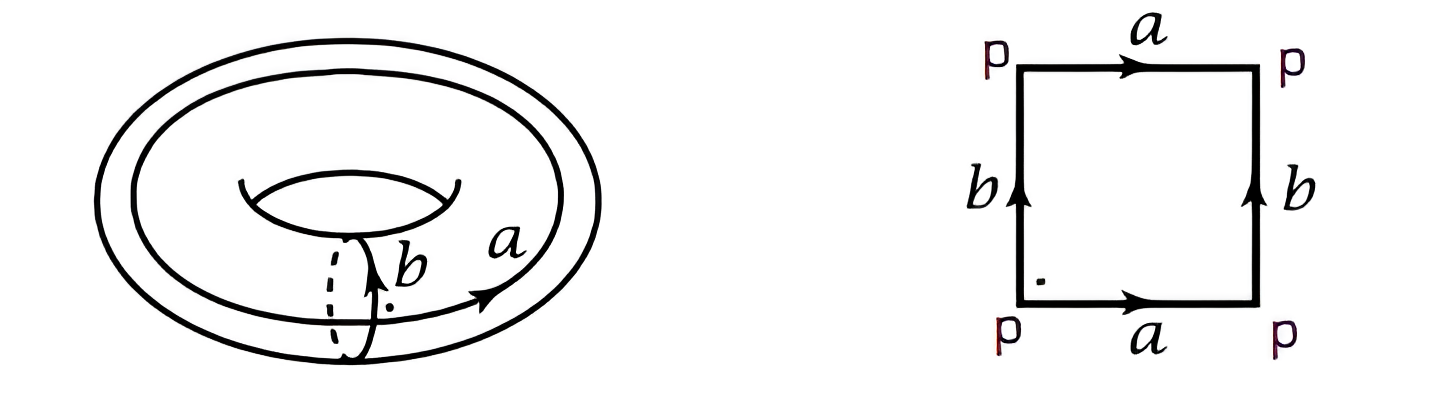
\includegraphics[height= 2.5cm]{torus.png}
    \caption{The torus $\mathbb{T}^2$ and its presentation as a cell complex (source: \cite{hatcher})}
    \label{fig:torus}
  \end{center}
\end{figure}
\\
In HoTT, this suggests the following definition by a HIT where we would manually fill the square:
\begin{itemize}
  \item $ p : \mathbb{T}^2$
  \item $a : p = p$
  \item $b : p = p $
  \item $\mathrm{fill} :  a \cdot b = b \cdot a$
\end{itemize}
And, thanks to square types in cubical theory we can also give the following definition (in the cubical agda syntax, which should be readily understandable) : 
\begin{lstlisting}[mathescape=true]
    data Torus2 : Type where
    p : Torus2
    a : $ p \equiv p$
    b : $p \equiv p$
    fill : Square b b a a
\end{lstlisting}
Similarly, one can fill cubes in cubical type theory, but the structures involved quickly gain in complexity (we will look at such cubes a bit later).
\chapter{The Hypercubic manifold} 
In this part, we will cover the work on the \textbf{hypercubic manifold} done during the internship. The formalized proofs and attempts of proofs can be found on the following GitHub repository \cite{repo}. \\
Section 5 comes from my own work during the internship. Section 6 is a check made during the internship to verify the coherence of section 5, so it contains no new results. Section 7 was a more in depth calculation of a side question my advisors had on a object they are working on and that is a good starting point for the calculations that come afterwards. Section 8 contains personal work from the internship, not yet completed, but was the second goal of the internship (after the result in section 5).
\section{Defining the hypercubic manifold}
The first part of the work was to give a formalised definition of the \textbf{hypercubic manifold}. This manifold can be obtained as the adjunction space of a 3-dimensional hypercube where opposite sides are identified with a quarter turn rotation. This is best illustrated in the following video \cite{VHvideo}. It can be presented as the following object (illustration taken from \cite{hypercubic}):
\begin{figure}[h]
  \begin{center}
    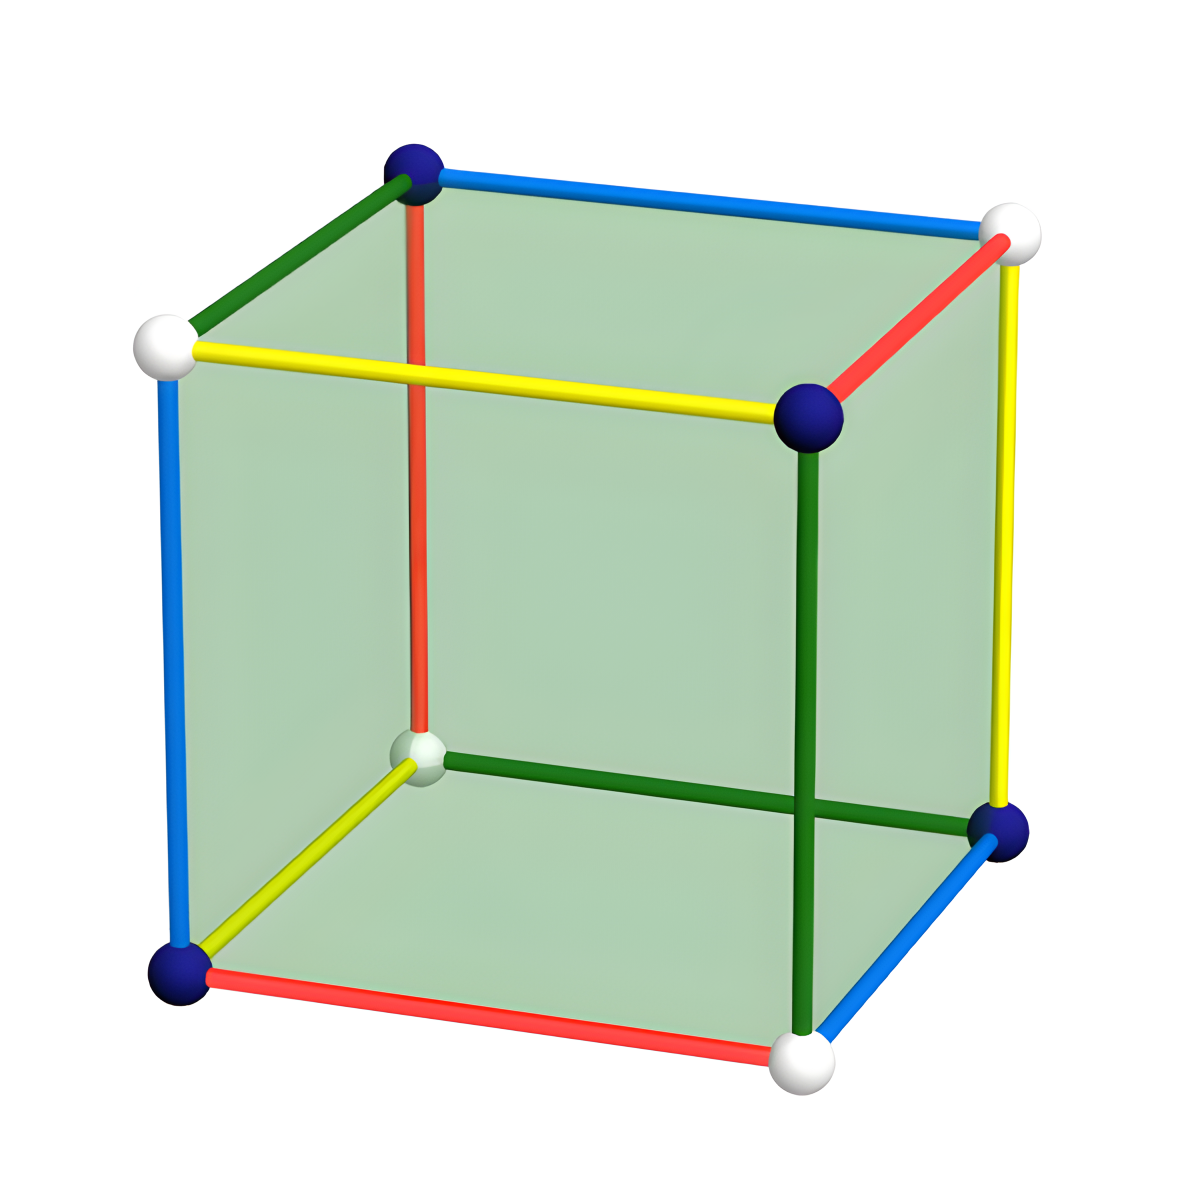
\includegraphics[height= 6.5cm]{cube-3-2.png}
    \caption{The hypercubic manifold}
    \label{fig:H1M}
  \end{center}
\end{figure}\\
Our goal is to define this object as a HIT, since we can already see what vertices and edges should be there. There are a few things that should be kept in mind however. First, this HIT would require filling a cube which can be a little tricky. Then, opposite faces are actually the same up to a quarter turn rotation so this should also be sorted out within our HIT (this kind of structure did not appear for the circle or the torus we previously saw). It should also be noted that filling squares is feasible in HoTT since it is tantamount to a commuting square of paths. However, filling cubes ought to be much more complicated since it deals with relations on squares. This is where cubical type theory is hoped to come in handy.\\
So, the first part of the work during this internship was to comprehend the specificities of cubical type theory, becoming more familiar with filling squares and cubes, so as to be able to tackle the more complex case of the hypercubic manifold. To do so, I defined severaldifferent HITs involving increasingly difficult structures with squares, cubes or sides/edges being flipped to get as close as possible to our goal. All of these HITs can be found in the GitHub repository \cite{repo} in "HiTs.agda". 
\paragraph{The hypercubic manifold} To begin with, we will name the vertex constructors $b^V$ and $w^V$ (for blue and white vertex) and the edge constructors $b^E$, $r^E$, $g^E$, $y^E$ (for blue,red,green,yellow edges) as figure 2.1 suggests. Now, a filled square : 
\begin{center}
  \begin{tikzcd}
    {} \arrow[r, "s"]                 & {}                 \\
    {} \arrow[u, "p"] \arrow[r, "r"'] & {} \arrow[u, "q"']
  \end{tikzcd}
\end{center}
is tantamount to having a relation $p \cdot s \equiv r \cdot q$. The latter can be rewritten $r^{-1} \cdot p \equiv q \cdot s^{-1}$ which gives us a filled square : 
\begin{center}
  \begin{tikzcd}
    {} \arrow[r, "p"]                      & {}                      \\
    {} \arrow[u, "r^{-1}"] \arrow[r, "q"'] & {} \arrow[u, "s^{-1}"']
    \end{tikzcd}
\end{center}
This allows us to define a quarter of a turn rotation operation on squares (where $\overline{p}$ denotes path inversion in cubical agda): 
$$\text{rot : Square $p$ $q$ $r$ $s$ $\rightarrow$ Square $\overline{r}$ $\overline{s}$ $q$ $p$}$$
This function can be synthetically defined as the following : $\boxed{\text{rot sq $i$ $j$ $:\equiv$ sq $(\sim j)$ $i$}}$. This map is naturally a quasi equivalence since $\mathrm{rot}^4\equiv \mathrm{Id}$, and its inverse is a quarter turn rotation in the other direction.\\
We now have every ingredient to define the hypercubic manifold. We should first choose the orientation of our paths, which will all go from $w^V$ to $b^V$. Having chosen this direction, looking at the cubical documentation \cite{cubicalagda} (in Foundations/Prelude.agda) gives us the convention for filling cubes in agda, leading us to the following HIT:
\begin{figure}[h]
  \begin{center}
    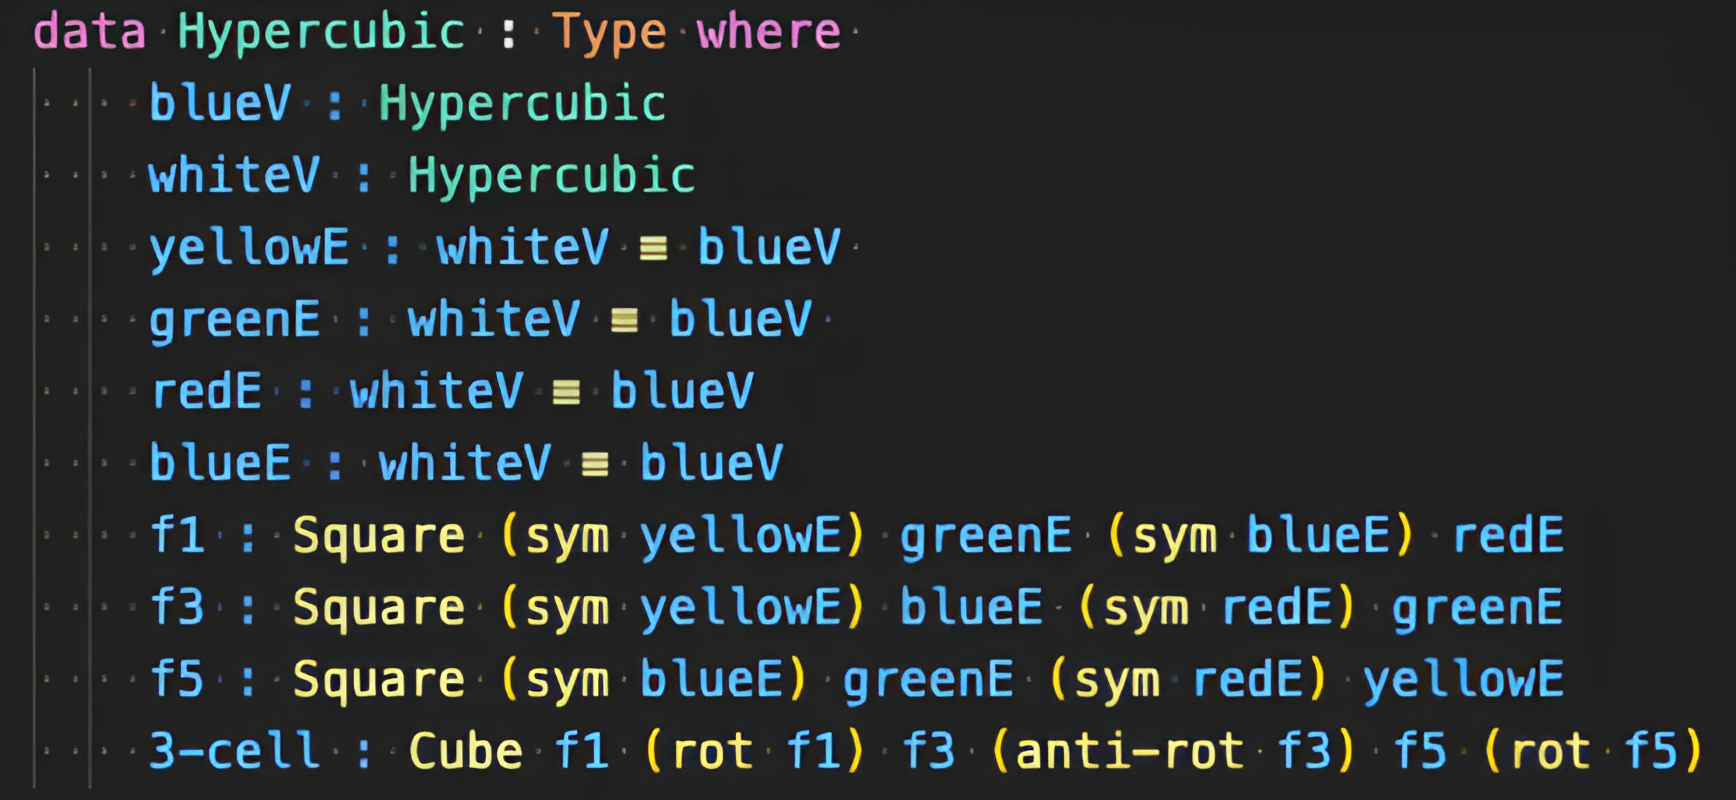
\includegraphics[height= 4.5cm]{images/Agda - VH.png}
    \caption{Synthetic description of the hypercubic manifold as a cubical HIT in cubical agda}
    \label{fig:H1Magda}
  \end{center}
\end{figure}\\
Having defined this HIT, that should indeed be the hypercubic manifold, we shall now be able to recover a known result about its fundamental group. We will denote the hypercubic manifold by $\mathbb{HM}^1$ from now on.
\section{The fundamental group of $\mathbb{HM}^1$}
\begin{theorem}
  We have that $\pi_1(\mathbb{HM}^1)=\mathcal{Q}$ where $\mathcal{Q}$ is the quaternion group.
\end{theorem}
Before proving this claim, we shall introduce a bit more \textbf{cell complexes} that we first saw in \ref{fig:torus}. A cell complex is a topological space built inductively by successively attaching $0$-cells (points), $1$-cells (paths) and so on. For small dimensions, one can give them an abstract presentation similar to the one of the torus \ref{fig:torus}. The way these spaces are built should remind of higher inductive types, where one specifies some point constructors ($0$-paths), then path constructors ($1$-paths) and so on. In section 6.6 of the HoTT book \cite{hott} one can find a further details about how a cell complex can be converted into a HIT. The idea is that attaching $n$-cells can be done by specifying algebraic relations (such as $p \cdot q = q \cdot p$ for the torus) on lower dimensional constructors. It appears that the represenation of $\mathbb{HM}^1$ in \ref{fig:H1M} is also a cell-complex representation and that the cubical definition in \ref{fig:H1Magda} is precisely its conversion into a HIT.\\
Now, in classical homotopy theory the fact that $\pi_1(\mathbb{HM}^1)=\mathcal{Q}$ is well known and follows from a corollary of the \textbf{Seifert Van Kampen} theorem, that states that the fundamental group of a cell complex is given by the fundamental group of its $2$-skeleton (that is, the complex where all cells of dimensions $>2$ are removed), more details can be found in \cite{hypercubic} and \cite{FundamentalCellComplex}. It can then be shown that the fundamental group of a cell complex with one $0$-cell is given by the presentation $\langle S \hspace{2pt} \vert\hspace{2pt} R \rangle$ where there is one generator in $S$ for every $1$-cell and one relation for any $2$-cell.\\
Now, the relations that the $2$-cells should give are precisely the one used when you convert a cell complex into a HIT so we can indeed check that the fundamental group of \ref{fig:H1Magda} is $\mathcal{Q}$ as it should be the case.\\
This verification took more time than expected because we had initillay overlooked the fact that the previous theorem applies to HITs with only one point constructors (the struggles we went through appear on the note we wrote \href{https://github.com/dlaird-ens/Stage-L3/blob/main/Rapport/annexes/hypercubic.pdf}{here}. The HIT in \ref{fig:H1Magda} gives us \textit{a priori} 4 generators $y,g,r,b$ (for the 4 paths constructors) and 3 relations (from the 3 filled squares that are tantamount to a commuting relation on paths, see \ref{fig:squarecommute}). After that, the presentation we obtained for the fundamental group of $\mathbb{HM}^1$ was the following (details can be found in the notes \href{https://github.com/dlaird-ens/Stage-L3/blob/main/Rapport/annexes/hypercubic.pdf}{here}, although some generators are inverted in this presentation and some relations have been rewritten from the ones you would normally obtain):
$$ \pi_1(\mathbb{HM}^1) = \langle r,g,b,y \quad \vert \quad by=rg, bgry=1, gb = yr \rangle$$
However, as stated before, this is not appropriate because we were working with two point constructors. The solution is to get back to a single point constructor by contracting one of the path constructors (-we chose to contract the yellow edge). This yields the presentation : 
$$ \pi_1(\mathbb{HM}^1) = \langle r,g,b \quad \vert \quad b=rg, bgr=1, gb = r \rangle$$
And this is a presentation of the quaternion group.
\begin{proof} The usual presentation for the quaternion group is given by : 
  $$\mathcal{Q}  = \langle e,i,j,k \quad \vert \quad i^2 =e, j^2=e, k^2=e, ijk=e, e^2=1 \rangle$$
  (If you are familiar with the usual quaternions, in this presentation $e$ should be thought of  playing the role of $-1$).
  Now we have to build a presentation isomorphism to show that these two groups are the same. In \href{https://github.com/dlaird-ens/Stage-L3/blob/main/Rapport/annexes/hypercubic.pdf}{his notes}, my advisor suggested using his tool that generates the \textbf{Knuth-Bendix} completion of a rewritting system to see what algebraic relations we could deduce from the presentation of $\pi_1(\mathbb{HM}^1)$. From those relations, it appears that $r,g,b$ are elements of order $4$, and so they should naturally identify to $k,j,i$, but since $bgr=1$ and $ijk=e(=-1)$, it is needed to identify one of the generators with the "opposite" of the other. The opposite is given by multiplying by an element of order $2$, so since $b$ is of order $4$ in $\pi_1(\mathbb{HM}^1)$, $bb$ is of order 2 and so can be used (non-canonically) to represent the minus sign. This lead to defining the following group isomorphisms (defining them actually involves a furtherprecautions, the full calculations are available \href{https://github.com/dlaird-ens/Stage-L3/blob/main/Rapport/annexes/Quaternions.pdf}{here}):\\\\
  \begin{minipage}{.5\textwidth} 
    $f : \pi_1(\mathbb{HM}^1) \rightarrow \mathcal{Q}$
    \begin{itemize}
      \item $f(r) := k$
      \item $f(g) := j$
      \item $f(b) :=ei$
    \end{itemize}
  \end{minipage}
  \hfill 
  \begin{minipage}{.5\textwidth} 
    $h : \mathcal{Q} \rightarrow \pi_1(\mathbb{HM}^1)$
    \begin{itemize}
      \item $h(i) := bbb$
      \item $h(j) := g$
      \item $h(k) := r$
      \item $h(e) :=bb$
    \end{itemize}
  \end{minipage}
\end{proof}
\section{A first fiber calculation}
Now, we have already encountered the \textbf{loop space} of a type $A$. A natural question is : given a pointed type $(A,a)$, does there exist a pointed type $(B,b)$ such that $\Omega(B,b)=(A,a)$ ? For a group $G$ (pointed at its unit element) the answer is yes and one can -easily- create such a space (it is done in \cite{cubicalagda} HITs/EilenbergMacLane1/Base.agda). We will call such a space a \textbf{delooping} of $G$ that we will note $\mathrm{B}G$ (in HoTT all deloopings are actually equal). The idea is to build a HIT with one point constructor $*$, a loop $p_g$ for every element $g$ in $G$ (this can be restrained to a set of generators of $G$) and add relations between those loops so that the group structure of the loop space at this point is the same as G (for instance, we want $p_g \cdot p_h \equiv p_{g.h} \cdot \mathrm{refl}$, and this is easily done in cubical type theory by filling squares). Using the arguments of the previous section, this yields the correct fundamental group, but we can't control what happens higher homotopy groups so we have to take the $1$-truncation of this type to kill off all the higher homotopy groups. This can be shown to indeed produce the loop space, but that is  not what will our aim. A famous theorem in algebraic topology (see \cite{hott}) is that $\mathrm{B}\mathbb Z = \mathbb{S}^1$.\\
Is is important to note that this construction uses a \textbf{1-truncation}, which is known to work theoretically but we really do not have a good understanding of what it actually does. We would then want to build some deloopings in a more "natural" or constructive way. Specifically, achieving a cellular delooping (that is, as a cell complex), would allow us to have some induction principles that are not restrained to $1$-types (as it was the case with the previous construction). This would then open up the possibility of defining some \textbf{higher group actions} (that is, not only on sets but also on $1$-types, $2$-types etc) and computing \textbf{cohomology} in the synthetic framework of HoTT and perhaps computer-check those calculations. In that regard, my advisors have a way to build such a delooping of the quaternion group $\mathcal Q$ from the hypercubic manifold $\mathbb{HM}^1$, but this whole construction relies on the calculation of the $\textbf{fiber}$ of a certain map, and this is what we will be looking at from now on. I will first start by exposing a preliminary calculation that I was given to do to get a grasp on the tools we have at hand. This calculation comes from some other work my advisors are doing on loop spaces of cyclic groups, for which they wanted to check one of their claims.
\begin{mydef}
  Let $f : A \rightarrow B$ be a map and $b : B$, we define the fiber of $f$ over $b$ by : 
  $$\mathrm{fib}_f(b) \hspace{3pt} :\equiv \sum_{x: A} f(x)=_B b$$
\end{mydef}
An interesting way to see the fiber of a map is via a pullback square \ref{fig:pullbacksquare}. For $b :B$ let $b_*$ be the map $\mathbf{1} \rightarrow B$ sending the canonical element $*$ to $b$. The the pullback of $f$ and $b_*$ is equivalent to the fiber $\mathrm{fib}_f(b)$ : 
\begin{center}
  \begin{tikzcd}
    \mathrm{fib}_f(b) \arrow[d] \arrow[r] & \textbf{1} \arrow[d, "b_*"] \\
    A \arrow[r, "f"']                                                  & B               
  \end{tikzcd}
\end{center}
This follows from the calculation : 
$$
A \times_B \textbf{1} :
\equiv \sum_{x :A} \sum_{y : \textbf{1}} f(x)=b_*(y)
\simeq \sum_{x : A} f(x)=b_*(*) 
:\equiv\mathrm{fib}_f(b)
$$
Let now $m$ be a nonnegative integer and $r \in \mathbb{Z}_m^{\times}$ (the integers mod $m$). Then we have a short exact sequence of groups : 
$$\mathbb{Z} \xrightarrow{\times m} \mathbb{Z} \xrightarrow{1 \mapsto \overline r} \mathbb Z_m$$
Which, for  topological reasons, yields a fibration of delooping spaces, where we identify $\mathrm{B}\mathbb Z$ and $\mathbb S^1$ as explained previously:
$$\mathbb{S}^1 \xrightarrow{\mathrm{base} \mapsto \mathrm{base}, \quad  \mathrm{loop} \mapsto \mathrm{loop}^m} \mathbb{S}^1 \xrightarrow{g} \mathrm{B}\mathbb{Z}_m$$
This is in fact a fibration whose base space is $\mathrm{B}\mathbb{Z}_m$, of total space $\mathbb{S}^1$, and for which the fiber of $g$ over the canonical element of $\mathrm{B}\mathbb{Z}_m$ should be $\mathbb{S}^1$ (we will actually prove this claim). Now, let $\mathrm{Fin} \hspace{2pt} m$ be the finite type with $m$ elements $0,\ldots, (m-1)$ and $s_m$ denote the equivalence of $\mathrm{Fin} \hspace{2pt} m$ given by $x\mapsto x+1 \pmod m$. From the work of my advisors, it appears that the connected component of $(\mathrm{Fin \hspace{2pt}, s_m})$ in the type of $\mathbb Z_m$ types (that is types equipped with an equivalence whose order is $m$) is a delooping of $\mathbb{Z}_m$ (this is specific to cyclic groups). One can ignore the domain of the equivalence (it is given implicitely) and so the connected component of $s_m$ is a delooping of $\mathbb Z_m$. Consequently, choosing this as a model of $\mathrm{B}\mathbb{Z}_m$, the map $g$ is given by : 
$$g(\mathrm{base}) :\equiv \mathrm{base}, \quad \mathrm{ap}_g(\mathrm{loop}) :\equiv \mathrm{ua}(s_m^r)$$
If $P : \mathrm{B}\mathbb{Z}_m \rightarrow \mathcal{U}$ is defined by $P :\equiv x \mapsto  x = s_m$ then we have a fibration over $\mathbb{S}^1$ given by $P \circ g$ whose total space is by definition:
$$\sum_{x : \mathbb{S}^1} P \circ g (x) :\equiv \sum_{x : \mathbb{S}^1}(g(x)=s_m) :\equiv \mathrm{fib}_g(s_m)$$ 
Now, as $\mathbb{S}^1$ is defined by the coequalizer diagram \ref{fig:coequalizer} :
\begin{center}
  \begin{tikzcd}
    1 \arrow[r, shift left] \arrow[r, shift right] & 1 \arrow[r, "\mathrm{base}"] & \mathbb{S}^1
  \end{tikzcd}
\end{center}
We obtain the following commuting diagram : 
\begin{center}
  \begin{tikzcd}
    1 \arrow[r, shift left] \arrow[r, shift right] & 1 \arrow[r, "\mathrm{base}"] \arrow[rd, "s_m =s_m"'] & \mathbb{S}^1 \arrow[r, "g"] \arrow[d, "P \circ g" description] & \mathrm{B} \mathbb{Z}_m \arrow[ld, "P"'] \\
                                                   &                                                      & \mathcal U                                                     &                                         
  \end{tikzcd}
\end{center}
So, we went from calculating the fiber of a map to calculating the total space of a fibration over a space which is defined as a coequalizer. This is convenient since we have a lemma that allows us to calculate total spaces of fibrations over coequalizers in a convenient way : 
\begin{prop}[Flattening Lemma]
  Suppose given a fibration over a coequalizer type: 
  \begin{center}
    \begin{tikzcd}
      B \arrow[r, "f", shift left] \arrow[r, "g"', shift right] & A \arrow[r, "c"] & W \arrow[r, "P"] & \mathcal U
    \end{tikzcd}
  \end{center}
  Then, one has a coequalizer diagram between the total spaces: 
  \begin{center}
    \begin{tikzcd}
      \displaystyle \sum_{b : B} P \circ c \circ f (a) \arrow[rrr, "{(b,x) \mapsto(g(b),p_b^*(x))}", shift left=3] \arrow[rrr, "{(b,x) \mapsto (f(b),x)}"', shift right=3] &  &  & \displaystyle \sum_{a : A} P \circ c (a) \arrow[rr] &  & \displaystyle \sum_{w : W} P(w)
    \end{tikzcd}
  \end{center}
\end{prop}
In our case, the lemma yields the following coequalizer diagram :
\begin{center}
\begin{tikzcd}
  s_m=s_m \arrow[rr, "\mathrm{Id}", shift left] \arrow[rr, "p \mapsto p^r"', shift right] &  & s_m=s_m \arrow[r] & \mathrm{fib}_g(s_m)
\end{tikzcd}
\end{center}
Given that $(s_m = s_m) \simeq (s_m \simeq s_m) \simeq \langle s_m \rangle \simeq \mathrm{Fin} \hspace{2pt} m$ , we get that $\mathrm{fib}_g(s_m)$ is equivalent to the HIT $W$ defined by the following constructors : 
\begin{itemize}
  \item $c : \mathrm{Fin} \hspace{2pt} m \mapsto W$
  \item $ p : \prod_{x : \mathrm{Fin}\hspace{2pt} m} (c(x) = c(s_m^r(x)))$
\end{itemize}
Since $r$ is coprime to $m$, it turns out that $s_m^r$ is of order $m$ so the orbit of $c(0)$ under the action of the group $\langle s_m^r \rangle$ is the whole type $W$, taking the example of $r=1$ and $m=4$ one gets the following type :
\begin{center}
  \begin{tikzpicture}[scale=0.55]
    \draw (-2,0.5) .. controls (-2,1) and (-1,2) .. (-0.5,2) node [midway, above left] {$p_0$};
    \draw (0.5,2) .. controls (1,2) and (2,1) .. (2,0.5) node [midway, above right] {$p_1$};
    \draw (2,-0.5) .. controls (2,-1) and (1,-2) .. (0.5,-2) node [midway, below right] {$p_2$};
    \draw (-0.5,-2) .. controls (-1,-2) and (-2,-1) .. (-2,-0.5) node [midway, below left] {$p_3$};
    \node (A) at (-2,0) {$c(0)$};
    \node (A) at (0,2) {$c(1)$};
    \node (A) at (2,0) {$c(2)$};
    \node (A) at (0,-2) {$c(3)$};
  \end{tikzpicture}
\end{center}
And this is equivalent to the circle $\mathbb{S}^1$. By univalence we then have :
$$\boxed{\mathrm{fib}_g(s_m) = \mathbb{S}^1}$$
We will not set out the proof of the equivalence in detail (it can be found in an annex \href{https://github.com/dlaird-ens/Stage-L3/blob/main/Rapport/annexes/Fibre.pdf}{here}), but the idea is that the general case should come from the case $r=1$, and for $r=1$, we have that $p_0 \cdot p_1 \cdot \ldots \cdot p_m : c(0)=c(0)$ and we can successively contract each path $p_i : c(i)\rightarrow c(\overline{i+1}_r)$, to end up with a type with a constructor $c(0)$ and a path $p_0 : c(0) = c(0)$, which is the circle. \\\\
I also proved an extension of this result (also in the annex) to the case where $r$ and $m$ are not coprime. In that case, let $\delta$ be the $\gcd$ of $r$ and $m$, then $s_m^r$ is now only of order $\frac m{\delta}$, and so our type is composed of $\delta$ disjoint orbits of size $\frac m{\delta}$, each orbit looking like the types we were previously looking at. We then naturally obtain : 
$$\boxed{\mathrm{fib}_g(s_m) = \bigplus_{i=1}^{\delta} \mathbb{S}^1}$$
\section{Towards $\mathbb{HM}^1$ as a quotient of $\mathbb{S}^3$ under an action of $\mathcal{Q}$}

\begin{mydef}
  An action of a group $G$ on a type $A$ is a map $f : \mathrm{B}G \rightarrow \mathcal{U}$ such that $f(*) :\equiv A$, where $*$ is the canonical element of $\mathrm{B}G$.
\end{mydef}
Let us consider the case where $A$ is a set to recover usual group actions. Given $f : \mathrm{B}G \rightarrow \mathcal{U}$ such that $f(*) :\equiv A$ then the induction principle for $\mathrm{B}G$ tells us that every loop from $(*=*) \simeq G$ has to be sent to an element of $A=A$, and by univalence to an equivalence of $A$. Hence, via the identification of $*=*$ to $G$, we have sent every element $g$ of $G$ to an equivalence of $A$ , as expected for a group action. Moreover, we have stated the fact that $f$ behaves \textbf{functorially} on paths, meaning that for two paths $g,h : G$ we have $f(g \cdot h) = f(g) \cdot f(h)$ and $f(e_G)=\mathrm{refl}_A$, which are the axioms for a group action. \\\\
It is known in homotopy theory that $\mathbb{HM}^1$ is the quotient of the sphere $\mathbb{S}^3$ by an action of the quaternion group $\mathcal{Q}$ (see \cite{hypercubic}). This is indeed given by a certain map $f : \mathbb{HM}^1 \rightarrow \mathrm{B} \mathcal{Q}$. Given such a map, one has that: 
$$\mathrm{fib}_f(*) = \sum_{x : \mathbb{HM}^1} (f(x) = *)$$
Then by connectedness, $(f(x)=*) \simeq (*=*) \simeq \mathcal{Q}$ for any $x : \mathbb{HM}^1$, meaning that $\mathcal{Q}$ operates transitively on every fiber $f(x)=*$, which at turns yields an action of $\mathcal{Q}$ on $\mathrm{fib}_f(*)$, transitive on every fiber and so the quotient under the action of $\mathcal{Q}$ is then naturally equivalent to $X$. This means that such a map expresses $X$ as a homotopy quotient of $\mathrm{fib}_f(*)$ under an action of $Q$. Hence, by defining the correct map we are to expect that $\mathrm{fib}_f(*) = \mathbb{S}^3$. In our case the map is given by (we identify $\pi_1(\mathrm{B}\mathcal Q)$ and $\mathcal{Q}$ and since $\mathrm{B}\mathcal{Q}$ is 1-truncated we need not specify its values on the $2$-cells and $3$-cells):
$$f : \mathbb{HM}^1 \rightarrow \mathrm{B} \mathcal{Q},\hspace{2pt} f(b^V) \equiv f(w^V) :\equiv *,\hspace{2pt} f(y^E):\equiv 1_{\mathcal{Q}}, f(g^E):\equiv j,f(r^E):\equiv -k, f(b^E):\equiv i. $$ 
To compute this fiber, we will use the same technique as before by defining $P : \mathrm{B} \mathcal Q \rightarrow \mathcal U$ by $P :\equiv x \mapsto x=*$. Then the fiber is obtained as the total space of the fibration $P \circ f $ over $\mathbb{HM}^1$. Here, we can express $\mathbb{HM}^1$ as a (triple) pushout, and since we have a flattening lemma that also holds for pushout types we should be able to effectively compute what we want. The 3 pushouts encompass precisely how we successively build the 1-skeleton, 2-skeleton, 3-skeleton. They are given by the following three diagrams : 
\begin{center}
  \begin{tikzcd}
    \mathrm{edges} \arrow[d, "\mathrm{source}"'] \arrow[r, "\mathrm{target}"] & b^V \arrow[d] \arrow[ld, Rightarrow] &  & 3\mathbb{S}^1 \arrow[d, "f"'] \arrow[r, "g"] & \mathrm{sides} \arrow[d] \arrow[ld, Rightarrow] &  & \mathbb{S}^2 \arrow[d,"h"'] \arrow[r,"k"] & \mathrm{fill} \arrow[d] \arrow[ld, Rightarrow] \\
    w^V \arrow[r]                                                             & 1\mathrm{Sk}                         &  & 1\mathrm{Sk} \arrow[r]                       & 2\mathrm{Sk}                                    &  & 2\mathrm{Sk} \arrow[r]           & 3\mathrm{Sk}                                  
  \end{tikzcd}
\end{center}
More details on their definition can be found on the GitHub repository \cite{repo} (in 1Skeleton.agda, 2SkeletonCircle.agda and 3Skeleton.agda). \\
We will now take a closer look at the 1-skeleton. The type $\mathrm{edges}$ is defined to be the set with $4$ elements $b^E,r^E,y^E,g^E$. Hence the pushout type $1\mathrm{Sk}$ is given by two points constructors $\mathrm{inl}(w^V)$ and $\mathrm{inr}(b^V)$ and 4 edges between them $\mathrm{glue}(b^E)$,$\mathrm{glue}(r^E)$,$\mathrm{glue}(y^E)$,$\mathrm{glue}(g^E)$. It is readily verified that this is indeed the 1-skeleton of our hypercubic manifold \ref{fig:H1Magda}. For that level, the file 1Skeleton.agda actually contains a proof of an equivalence between this pushout and the 1-skeleton. \\
Now, the goal of my work was to compute the fiber of the previous map, which requires a three-folded application of the flattening lemma. Moreover, the combinatorial nature of the objects at stake here is such, that manipulating their induction principles that may contain paths, dependant paths and paths over paths is already quite difficult by itself. This is why I used to the agda proof assistant to complete this part of the work. Moreover, since we are filling squares and cubes, cubical type theory should be convenient for that purpose. A first step to be actually able to use the flattening lemma in agda (it has already been proven in the cubical agda library \cite{cubicalagda}) was to define those 3 pushouts and make sure that we obtain a type that is equivalent to the one we previously defined. Defining them is a relatively easy task, the question of the equivalences is however much harder to formalise using a proof assistant. \\
As of now, I still do not have satisfactory results for the 2-skeleton and 3-skeleton. The part I spent most time on was the 2 Skeleton. In my GitHub repository there a few different files for the 2-skeleton. Those exist because we were trying different models of the circle and the type $\mathrm{sides}$ to define our pushouts. On the one hand, we could have gone with a squared model of the circle and a filled squared model for the sides. This has the advantage of being easily translated from our original type. There are, however two problems. First these types are much more complex, so the flattening lemma will not help us much (it is useful when we obtain total spaces over small types such as the unit type since they compute pretty easily). Second, is a problem coming from the proof assistant itself. In short, in this model we would fill some squares that are then injected through the right side in our 2-skeleton, when we would want them injected from the left side. Correcting this problem involves some complicated transport operations and so I dropped this model.\\
Afterwards , we decided to go with a point model for sides and the usual circle, this is what is done in 2SkeletonCircle.agda, this is much more synthetic so should fit the flattening lemma better, and it seems that the transporting operations are much easier since we can reconvert them into path relations, as previously seen. The file PathLemmas.agda contains some paths lemmas that are nearly sufficient to succeed in one transport operation that we previously could not do, so it appears that we are moving in the right direction.\\
\section*{Conclusion} 
During this internship I gained a lot of theoretical knowledge about a broad range of topics (categories, homotopy theory, type theory), that were at the basis of all the work done afterwards. Moreover, I also learnt a lot on the proof assistant agda, and experienced firshand the struggle to convert what we know and have a proof of into a computer-checked proof. In terms of production, I was satisfied with how I completed what is presented in part 5,6 and 7. However, what should have been the 'icing on the cake' in section 8 took much more time than I had thought it would and, unfortunately, I was not able to complete it in time (it should hopefully be completed in the near future).
\addcontentsline{toc}{chapter}{Conclusion}
\renewcommand\bibname{Bibliography and links}
\printbibliography
\section*{Context}
My internship was supervised by Samuel Mimram and Emile Oleon who are members of the Cosynus team at the LIX (Laboratoire d'informatique de l'Ecole Polytechnique). This team works on topics such as categories, directed algebraic topology, proofs and semantics. The offices of the Cosynus team were in the same corridor as the AlCo team (Algorithms and Complexity), and so both teams usually share the lunch break. There were several PhD students present there with whom I talked about studies, upcoming internships and life as a doctoral student. These conversations gave me some very incisive insights. The LIX is much bigger than those two teams alone and shares its building with INRIA Saclay, so there was a large number of people working there. I found that it was interesting to learn more about how a lab actually works (with all the administrative duties aswell), and to see how differently teams can operate within the same lab.
\end{document}
